\documentclass[a4paper, 12pt, addpoints]{exam}
\usepackage{IfbaListas}
%==============================================================
\NumList{1} %NÚMERO DA LISTA
\Assunto{Lógica Proposicional}
%==============================================================
%=========================================================
%------------Cabeçalho e rodapé 
%=========================================================
\pagestyle{headandfoot}%{head}%empty
\firstpageheader{}{}{}
\runningheader{\disciplina}{}{Lista \numlist: \assunto}
\runningheadrule
% \copyright \professor
\firstpagefooter{}{}{Pag. \thepage\ de \numpages}
%\iflastpage{Outros templates em \href{http://gg.gg/profwaldexsantos}{gg.gg/profwaldexsantos}
\runningfooter{}{}{Pag. \thepage\ de \numpages}
\runningfootrule
%===============================================================
%INFORMAÇÕES SOBRE A AVALIAÇÃO
\nomeInst{Instituto Federal da Piauí}
\logoInst{
\includegraphics[scale=0.17]{Figs/IFPIPicosVertical.png}}
\Campus{Picos} %PARA ENSINO FUNDAMENTAL OU MÉDIO-COMENTE ESTA LINHA COM %
\nomeCurso{Análise e Desenvolvimento de Sistemas} %Se não for curso superior, basta comentar esta linha ou deixar em branco
\nomeDisciplina{Matemática Computacional}
\Semestre{1}
\nomeProfessor{Rogerio Figueredo de Sousa}
\Aluno{}
\matriculaAluno{}
%===============================================================
 %CARREGA AS INFORMAÇÕES GERAIS DO PROFESSOR, ESCOLA ETC
%==============================================================

%COMEÇO DO DOCUMENTO
\begin{document}
\info\vspace{-1 cm} %Imprime as informações do cabeçalho programada no pacote 
% inicia a gravacao da resposta no arquivo "ans" cujo nome externo é gabarito 
\Opensolutionfile{ans}[Gabarito]
%*****************************************************************************
\begin{questions}%COMEÇA O AMBIENTE DE QUESTÕES
  \question São dadas diversas formas de negação para cada uma das proposições a seguir.
  Quais estão corretas?

  \begin{enumerate}[a)]
    \item  A resposta é 2 ou 3.
          \begin{enumerate}[i.]
            \item A resposta é nem 2 nem 3.
            \item A resposta não é 2 ou não é 3.
            \item A resposta não é 2 e não é 3.
          \end{enumerate}
    \item Pepinos são verdes e têm sementes.
          \begin{enumerate}[i.]
            \item Pepinos não são verdes e não têm sementes.
            \item Pepinos não são verdes ou não têm sementes.
            \item Pepinos são verdes e não têm sementes.
          \end{enumerate}
    \item $ 2 < 7 $ e $3$ é ímpar.
          \begin{enumerate}
            \item $2 > 7$ e 3 é par.
            \item $2 \geq 7$ e 3 é par.
            \item $2 \geq  7$ ou 3 é ímpar.
            \item $2 \geq  7$ ou 3 é par.
          \end{enumerate}
  \end{enumerate}

  \begin{resp}~
    \begin{multicols}{4}
          \begin{enumerate}[a)]
            \item i e iii
            \item ii
            \item iv
          \end{enumerate}
        \end{multicols}
  \end{resp}

  \question  Qual é o valor lógico (V ou F) de cada uma das proposições a seguir?
  \begin{multicols}{2}
    \begin{enumerate}[a)]
      \item Se 8 for ímpar, então 6 é ímpar.
      \item Se 8 for par, então 6 é ímpar.
      \item Se 8 for ímpar, então 6 é par.
      \item Se 8 for ímpar e 6 for par, então 8 < 6.
    \end{enumerate}
  \end{multicols}

  \begin{resp}~
    \begin{multicols}{4}
      \begin{enumerate}[a)]
        \item V
        \item F
        \item V
        \item V
      \end{enumerate}
    \end{multicols}
  \end{resp}

  \question  Encontre o antecedente e o consequente de cada uma das proposições a seguir:

  \begin{enumerate}[a)]
    \item O crescimento sadio de plantas é consequência de quantidade suficiente de
          água.
    \item O aumento da disponibilidade de informação é uma condição necessária para
          um maior desenvolvimento tecnológico.
    \item Serão introduzidos erros apenas se forem feitas modificações no programa.
    \item A economia de energia para aquecimento implica boa insulação ou vedação
          de todas as janelas.
  \end{enumerate}

  \begin{resp}~
    %\begin{multicols}{4}
        \begin{enumerate}[a)]
          \item \textbf{antecedente:} água suficiente \\ \textbf{consequente:} crescimento saudável da planta
          \item \textbf{antecedente:} maior desenvolvimento tecnológico \\ \textbf{consequente:} aumento da disponibilidade da informação
          \item \textbf{antecedente:} erros serão introduzidos \\ \textbf{consequente:} haver uma modificação no programa
          \item \textbf{antecedente:} economia de energia \\ \textbf{consequente:} boa insulação ou vedação de todas as janelas
        \end{enumerate}
     % \end{multicols}
  \end{resp}

  \question Escreva a negação de cada fbf a seguir:
  \begin{enumerate}[a)]
    \item Se a comida é boa, então o serviço é excelente.
    \item Ou a comida é boa, ou o serviço é excelente.
    \item Ou a comida é boa e o serviço é excelente, ou então está caro.
    \item Nem a comida é boa, nem o serviço é excelente.
    \item Se é caro, então a comida é boa e o serviço é excelente.
  \end{enumerate}

  \begin{resp}~
       %\begin{multicols}{1}
        \begin{enumerate}[a)]
          \item A comida é boa mas o serviço é ruim.
          \item A comida e o serviço são ruins.
          \item A comida é ruim ou o serviço é ruim, mas o preço é baixo.
          \item A comida é boa ou o serviço é excelente.
          \item O preço é alto, mas a comida é ruim ou o serviço é ruim.
        \end{enumerate}
      %\end{multicols}
  \end{resp}

  \question Sejam A, B e C as seguintes proposições:
  \begin{enumerate}[A -]
    \item Rosas são vermelhas.
    \item Violetas são azuis.
    \item Açúcar é doce.
  \end{enumerate}

  Escreva as proposições compostas a seguir em notação simbólica.

  \begin{enumerate}[a)]
    \item Rosas são vermelhas e violetas são azuis.
    \item Rosas são vermelhas e, ou bem violetas são, ou bem açúcar é doce.
    \item Sempre que violetas são azuis, rosas são vermelhas e açúcar é doce.
    \item Rosas são vermelhas apenas se violetas não forem azuis ou se açúcar for
          amargo.
    \item Rosas são vermelhas e, se açúcar for amargo, então ou violetas não são azuis
          ou açúcar é doce.
  \end{enumerate}

  \begin{resp}~
    \begin{multicols}{3}
      \begin{enumerate}[a)]
        \item $A \wedge B$
        \item $A \wedge (B \vee C)$
        \item $B \rightarrow (A \wedge C)$
        \item $A \rightarrow (B' \vee C')$
        \item $A \wedge [C' \rightarrow (B' \vee C)]$
      \end{enumerate}
    \end{multicols}
    %\[ A \wedge (B \rightarrow C) \wedge \left[ (A \wedge B) \rightarrow (D \vee C') \right] \wedge B \rightarrow D \]
  \end{resp}


  \question Use A, B e C como no exercício 5 para escrever as seguintes proposições compostas
  em português:
  \begin{multicols}{2}
    \begin{enumerate}[a)]
      \item $B \vee C'$
      \item $B' \vee (A \rightarrow C)$
      \item $(C \wedge A') \leftrightarrow B$
      \item $C \wedge (A' \leftrightarrow B)$
      \item $(B \wedge C')' \leftrightarrow A$
      \item $A \vee (B \wedge C')$
      \item $(A \vee B) \wedge C'$
    \end{enumerate}
  \end{multicols}

  \begin{resp}~
    
      \begin{enumerate}[a)]
        \item Violetas são azuis ou açúcar é amargo.
        \item Violetas não são azuis ou, se rosas são vermelhas então o açúcar é doce.
        \item O açúcar é doce e rosas não são vermelhas se, e somente se, violetas são
        azuis.
        \item O açúcar é doce e, rosas não serem vermelhas é uma condição necessária e
        suficiente para violetas serem azuis.
        \item Se é falso que violetas são azuis e que açúcar é amargo, então rosas são
        vermelhas.
        \item As rosas são vermelhas ou, violetas são azuis e o açúcar é amargo.
        \item As rosas são vermelhas ou violetas são azuis, mas o açúcar é amargo.
      \end{enumerate}
    
  \end{resp}

  \question Escreva cada uma das proposições compostas a seguir em notação simbólica usando
  letras de proposição para denotar as componentes.

  \begin{enumerate}[a)]
    \item Se os preços subirem, então haverá muitas casas para vender e elas serão
          caras; mas se as casas não forem caras, então, ainda assim, haverá muitas casas para
          vender.
    \item Tanto ir dormir como ir nadar é uma condição suficiente para a troca de roupa;
          no entanto, mudar a roupa não significa que se vai nadar.
    \item Vai chover ou nevar, mas não ambos.
    \item Se Jane vender ou perder, vai ficar cansada.
    \item Ou Jane irá vender ou, se perder, ela ficará cansada.
  \end{enumerate}

  \begin{resp}~
    \begin{enumerate}[a)]
      \item A - Preços subirem; B - Haverá muitas casas para vender; C - As casas serão caras; \\ $ A \rightarrow (B \wedge C) \wedge (C' \rightarrow B) $
      \item A - Ir dormir; B - Ir nadar; C - Trocar de roupa \\ $[(A \vee B) \rightarrow C] \wedge (C \rightarrow B)'$
      \item A - Vai chover; B - Vai nevar. \\ $(A \vee B) \wedge (A \wedge B)'$ ou $ A \veebar B $
      \item A - Jane vai vender; B - Jane vai perder; C - Jane vai ficar cansada. \\ $(A \vee B) \rightarrow C$
      \item A - Jane vai vender; B - Jane vai perder; C - Jane vai ficar cansada. \\ $A \vee (B \rightarrow C)$
      
    \end{enumerate}
  \end{resp}

  \question Escreva cada uma das proposições compostas a seguir em notação simbólica usando
  letras de proposição para denotar as componentes.

  \begin{enumerate}[a)]
    \item Se o cavalo estiver descansado, o cavaleiro vencerá.
    \item O cavaleiro vencerá apenas se o cavalo estiver descansado e a armadura for
          forte.
    \item Um cavalo descansado é uma condição necessária para o cavaleiro vencer.
    \item O cavaleiro vencerá se, e somente se, a armadura for forte.
    \item Uma condição suficiente para o cavaleiro vencer é que a armadura seja forte
          ou o cavalo esteja descansado.
  \end{enumerate}

  \begin{resp}~

    Prop.: A - Cavalo estiver descansado; B - Cavaleiro vencerá; C - Armadura é forte
    
    \begin{multicols}{4}
    \begin{enumerate}[a)]
      \item $ A \rightarrow B$
      \item $B \rightarrow (A \wedge C)$
      \item $B \rightarrow A$
      \item $B \leftrightarrow C$
      \item $(C \vee A) \rightarrow B$
    \end{enumerate}
  \end{multicols}
  \end{resp}

  \question Construa tabelas-verdade para as fbfs a seguir. Note quaisquer tautologias,
  contradições e contingências.
  \begin{multicols}{2}
    \begin{enumerate}[a)]
      \item $(A \rightarrow B) \leftrightarrow A' \vee B$
      \item $(A \wedge B) \vee C \rightarrow A \wedge (B \vee C)$
      \item $A \wedge (A' \vee B')'$
      \item $A \wedge B \rightarrow A'$
      \item $(A \rightarrow B) \rightarrow [(A \vee C) \rightarrow ( B \vee C)]$
      \item $A \rightarrow (B \rightarrow A)$
      \item $A \wedge B \leftrightarrow B' \vee A'$
      \item $(A \vee B') \wedge (A \wedge B)'$
      \item $[(A \vee B) \wedge C'] \rightarrow A' \vee C$
    \end{enumerate}
  \end{multicols}
  \begin{resp}~

    \begin{enumerate}[a)]
      \item Tautologia \\
      \begin{tabular}{|c|c|c|c|c|c|c|}
        \hline
        A & B & $ A' $ & $A \rightarrow B$ & $A' \lor B$ & $(A \rightarrow B) \leftrightarrow \lnot A \lor B$ \\
        \hline
        V & V & F & V & V & V \\
        V & F & F & F & F & V \\
        F & V & V & V & V & V \\
        F & F & V & V & V & V \\
        \hline
      \end{tabular}
      
      \item Contingência \\
      \begin{tabular}{|c|c|c|c|c|c|c|c|c|c|}
        \hline
        A & B & C & $(A \land B)$ & $(A \land B) \lor C$ & $(B \lor C)$ & $A \land (B \lor C)$ & $(A \land B) \lor C \rightarrow A \land (B \lor C)$ \\
        \hline
        V & V & V & V & V & V & V & V \\
        V & V & F & V & V & V & V & V \\
        V & F & V & F & V & V & V & V \\
        V & F & F & F & F & F & F & V \\
        F & V & V & F & V & V & F & F \\
        F & V & F & F & F & V & F & V \\
        F & F & V & F & V & V & F & F \\
        F & F & F & F & F & F & F & V \\
        \hline
      \end{tabular}
      
      \item Contingência \\
      \begin{tabular}{|c|c|c|c|c|c|c|}
        \hline
        A & $A'$ & $B'$ & $A' \lor B'$ & $(A' \lor B')'$ & $A \land (A' \lor B')'$ \\
        \hline
        V & F & F & F & V & V \\
        V & F & V & V & F & F \\
        F & V & F & V & F & F \\
        F & V & V & V & F & F \\
        \hline
      \end{tabular}

      \item Contingência \\
      \begin{tabular}{|c|c|c|c|c|c|}
        \hline
        A & B & $A'$ & $A \land B$ & $(A \land B) \rightarrow A'$ \\
        \hline
        V & V & F & V & F \\
        V & F & F & F & V \\
        F & V & V & F & V \\
        F & F & V & F & V \\
        \hline
      \end{tabular}

      \item Tautologia \\
      \resizebox{0.94\textwidth}{!}{%
      \begin{tabular}{|c|c|c|c|c|c|c|c|c|}
        \hline
        A & B & C & $(A \rightarrow B)$ & $(A \lor C)$ & $(B \lor C)$ & $[(A \lor C) \rightarrow (B \lor C)]$ & $(A \rightarrow B) \rightarrow [(A \lor C) \rightarrow (B \lor C)]$ \\
        \hline
        V & V & V & V & V & V & V & V \\
        V & V & F & V & V & V & V & V \\
        V & F & V & F & V & V & V & V \\
        V & F & F & F & V & F & F & V \\
        F & V & V & V & V & V & V & V \\
        F & V & F & V & F & V & V & V \\
        F & F & V & V & V & V & V & V \\
        F & F & F & V & F & F & F & V \\
        \hline
      \end{tabular}%
      }
      \item Tautologia \\
      \begin{tabular}{|c|c|c|c|}
        \hline
        A & B & $(B \rightarrow A)$ & $A \rightarrow (B \rightarrow A)$ \\
        \hline
        V & V & V & V \\
        V & F & V & V \\
        F & V & F & V \\
        F & F & V & V \\
        \hline
      \end{tabular}

      \item Contradição \\
      \begin{tabular}{|c|c|c|c|c|c|c|c|}
        \hline
        A & B & $A'$ & $B'$ & $A \land B$ & $B' \lor A'$ & $A \land B \leftrightarrow B' \lor A'$ \\
        \hline
        V & V & F & F & V & F & F \\
        V & F & F & V & F & V & F \\
        F & V & V & F & F & V & F \\
        F & F & V & V & F & V & F \\
        \hline
      \end{tabular}

      \item Contingência \\
      \begin{tabular}{|c|c|c|c|c|c|c|c|}
        \hline
        A & B & $B'$ & $(A \lor B')$ & $(A \land B)$ & $(A \land B)'$ & $(A \lor B') \land (A \land B)'$ \\
        \hline
        V & V & F & V & V & F & F \\
        V & F & V & V & F & V & V \\
        F & V & F & F & F & V & F \\
        F & F & V & V & F & V & V \\
        \hline
      \end{tabular}

      \item Contingência \\
      \begin{tabular}{|c|c|c|c|c|c|c|c|c|c|}
        \hline
        A & B & C & $A'$ & $C'$ & $(A \lor B)$ & $[(A \lor B) \land C']$ & $A' \lor C$ & $[(A \lor B) \land C'] \rightarrow A' \lor C$ \\
        \hline
        V & V & V & F & F & V & F & V & V \\
        V & V & F & F & V & V & V & F & F \\
        V & F & V & F & F & V & F & V & V \\
        V & F & F & F & V & V & V & F & F \\
        F & V & V & V & F & V & F & V & V \\
        F & V & F & V & V & V & V & V & V \\
        F & F & V & V & F & F & F & V & V \\
        F & F & F & V & V & F & F & V & V \\
        \hline
      \end{tabular}
    \end{enumerate}
  \end{resp}

  \question Nas sentenças a seguir que regra de inferência é ilustrada pelo argumento dado:
  \begin{enumerate}[a)]
    \item Se Martins é o autor, então o livro é de ficção. Mas o livro não é de ficção. Portanto,
          Martins não é o autor.
    \item Se a firma falir, todos os seus ativos têm que ser confiscados. A firma faliu. Segue
          que todos os seus bens têm que ser confiscados.
    \item O cachorro tem um pêlo sedoso e adora latir. Portanto, o cachorro adora latir.
    \item Se Paulo é um bom nadador, então ele é um bom corredor. Se Paulo é um bom
          corredor, então ele é um bom ciclista. Portanto, se Paulo é um bom nadador, então ele
          é um bom ciclista.
  \end{enumerate}

  \begin{resp}~
    
    \begin{multicols}{2}
      \begin{enumerate}[a)]
        \item Modus tollens
        \item Modus Ponens
        \item Simplificação
        \item Silogismo hipotético
      \end{enumerate}
    \end{multicols}
  \end{resp}

  \question Nas fbfs a seguir  use lógica proposicional para provar que o argumento é
  válido:

  \begin{enumerate}[a)]
    \item $A' \wedge (B \rightarrow A) \rightarrow B'$
    \item $(A \rightarrow B) \wedge [A \rightarrow (B \rightarrow C)] \rightarrow (A \rightarrow C)$
    \item $[(C \rightarrow D) \rightarrow C] \rightarrow [(C \rightarrow D) \rightarrow D]$
    \item $A' \wedge (A \vee B) \rightarrow B$
    \item $[A \rightarrow (B \rightarrow C)] \wedge (A \vee D') \wedge B \rightarrow (D \rightarrow C)$
    \item $(A' \rightarrow B') \wedge B \wedge (A \rightarrow C) \rightarrow C$
    \item $(A \rightarrow B) \wedge [B \rightarrow (C \rightarrow D)] \wedge [A \rightarrow (B \rightarrow C)] \rightarrow (A \rightarrow D)$
    \item $[A \rightarrow (B \rightarrow C)] \rightarrow [B \rightarrow (A \rightarrow C)]$
    \item $(A \wedge B) \rightarrow (A \rightarrow B')'$
  \end{enumerate}

  \begin{resp}~

    \begin{enumerate}[a)]
      \item $A' \wedge (B \rightarrow A) \rightarrow B'$ 
      \begin{multicols}{2}

        \begin{enumerate}[1.]
          \item $A'$
          \item $B \rightarrow A$
          \item $\boldsymbol{B'}$
        \end{enumerate}
        
        \columnbreak

        \begin{enumerate}[\ding{32}]
          \item (hip)
          \item (hip)
          \item \textbf{(1,2,modus tollens)}
        \end{enumerate}

        \end{multicols}

      \item $(A \rightarrow B) \wedge [A \rightarrow (B \rightarrow C)] \rightarrow (A \rightarrow C)$ \\
      \begin{multicols}{2}

        \begin{enumerate}[1.]
          \item $A \rightarrow B$
          \item $A \rightarrow (B \rightarrow C)$
          \item $A$
          \item $B$
          \item $B \rightarrow C$
          \item $\boldsymbol{C}$
        \end{enumerate}
        
        \columnbreak

        \begin{enumerate}[\ding{32}]
          \item (hip)
          \item (hip)
          \item (hip da conclusão)
          \item (1, 3, modus ponens)
          \item (2, 3, modus ponens)
          \item \textbf{(4, 5, modus ponens)}
        \end{enumerate}

      \end{multicols}
      
      \item $[(C \rightarrow D) \rightarrow C] \rightarrow [(C \rightarrow D) \rightarrow D]$ \\
      \begin{multicols}{2}

        \begin{enumerate}[1.]
          \item $(C \rightarrow D) \rightarrow C$
          \item $C \rightarrow D$
          \item $C$
          \item $\boldsymbol{D}$
        \end{enumerate}
        
        \columnbreak

        \begin{enumerate}[\ding{32}]
          \item (hip)
          \item (hip da conclusão)
          \item (1, 2, modus ponens)
          \item \textbf{(2, 3, modus ponens)}
        \end{enumerate}

      \end{multicols}
      
      \item $A' \wedge (A \vee B) \rightarrow B$ \\
      \begin{multicols}{2}

        \begin{enumerate}[1.]
          \item $A'$
          \item $A \vee B$
          \item $A'' \vee B$
          \item $A' \rightarrow B$
          \item $\boldsymbol{B}$
        \end{enumerate}
        
        \columnbreak

        \begin{enumerate}[\ding{32}]
          \item (hip)
          \item (hip)
          \item (2, dupla negação)
          \item (3, condicional)
          \item \textbf{(1, 4, modus ponens)}
        \end{enumerate}

      \end{multicols}

      \item $[A \rightarrow (B \rightarrow C)] \wedge (A \vee D') \wedge B \rightarrow (D \rightarrow C)$ \\
      \begin{multicols}{2}

        \begin{enumerate}[1.]
          \item $A \rightarrow (B \rightarrow C)$
          \item $A \vee D'$
          \item $B$
          \item $D$
          \item $A$
          \item $B \rightarrow C$
          \item $\boldsymbol{C}$
        \end{enumerate}
        
        \columnbreak

        \begin{enumerate}[\ding{32}]
          \item (hip)
          \item (hip)
          \item (hip)
          \item (hip da conclusão)
          \item (2, 4, silogismo disjuntivo)
          \item (1, 5, modus ponens)
          \item \textbf{(3, 6, modus ponens)}
        \end{enumerate}

      \end{multicols}
      
      \item $(A' \rightarrow B') \wedge B \wedge (A \rightarrow C) \rightarrow C$ \\
      \begin{multicols}{2}

        \begin{enumerate}[1.]
          \item $A' \rightarrow B'$
          \item $B$
          \item $A \rightarrow C$
          \item $A$
          \item $\boldsymbol{C}$
        \end{enumerate}
        
        \columnbreak

        \begin{enumerate}[\ding{32}]
          \item (hip)
          \item (hip)
          \item (hip)
          \item (1, 2, modus tollens)
          \item \textbf{(3, 4, modus ponens)} 
        \end{enumerate}

      \end{multicols}

      \item $(A \rightarrow B) \wedge [B \rightarrow (C \rightarrow D)] \wedge [A \rightarrow (B \rightarrow C)] \rightarrow (A \rightarrow D)$ \\
      \begin{multicols}{2}

        \begin{enumerate}[1.]
          \item $A \rightarrow B$
          \item $B \rightarrow (C \rightarrow D)$
          \item $A \rightarrow (B \rightarrow C)$
          \item $A$
          \item $B$
          \item $B \rightarrow C$
          \item $C$
          \item $C \rightarrow D$
          \item $\boldsymbol{D}$
        \end{enumerate}
        
        \columnbreak

        \begin{enumerate}[\ding{32}]
          \item (hip)
          \item (hip)
          \item (hip)
          \item (hip)
          \item (1, 4, modus ponens)
          \item (3, 4, modus ponens)
          \item (5, 6, modus ponens)
          \item (2, 5, modus ponens)
          \item \textbf{(7, 8, modus ponens)} 
        \end{enumerate}

      \end{multicols}

      \item $[A \rightarrow (B \rightarrow C)] \rightarrow [B \rightarrow (A \rightarrow C)]$ \\
      \begin{multicols}{2}

        \begin{enumerate}[1.]
          \item $A \rightarrow (B \rightarrow C)$
          \item $B$
          \item $A$
          \item $B \rightarrow C$
          \item $\boldsymbol{C}$
        \end{enumerate}
        
        \columnbreak

        \begin{enumerate}[\ding{32}]
          \item (hip)
          \item (hip da conclusão)
          \item (hip da hipótese da conclusão)
          \item (1, 3, modus ponens)
          \item \textbf{(2, 4, modus ponens)}
        \end{enumerate}

      \end{multicols}

      \item $(A \wedge B) \rightarrow (A \rightarrow B')'$ \\
      \begin{multicols}{2}

        \begin{enumerate}[1.]
          \item $A \wedge B$
          \item $A'' \wedge B''$
          \item $(A' \lor B')'$
          \item $\boldsymbol{(A \rightarrow B')'}$
        \end{enumerate}
        
        \columnbreak

        \begin{enumerate}[\ding{32}]
          \item (hip)
          \item (1, dupla negação)
          \item (2, De Morgan)
          \item \textbf{(3, condicional)}
        \end{enumerate}

      \end{multicols}

    \end{enumerate}
  \end{resp}


  \question Nas sentenças a seguir use lógica proposicional para provar que o argumento é
  válido. Use as letras de proposição dadas:

  \begin{enumerate}[a)]
    \item A colheita é boa, mas não há água suficiente. Se houver muita chuva ou se não
          houver muito sol, então haverá água suficiente. Portanto, a colheita é boa e há muito
          sol. C, A, V(chuva), S
    \item Se o anúncio for bom, o volume de vendas aumentará. O anúncio é bom ou a loja
          vai fechar. O volume de vendas não vai aumentar. Portanto a loja vai fechar. A, V, L
    \item A Rússia era uma potência superior e, a França não era suficientemente poderosa
          ou Napoleão fez um erro. Napoleão não fez um erro, mas, se o exército não perdeu,
          então a França era poderosa. Portanto, o exército perdeu e a Rússia era uma potência
          superior. R, F, N, E
    \item Não é verdade que, se as tarifas de energia elétrica subirem, então o uso diminuirá,
          nem é verdade que, novas usinas elétricas serão construídas ou as contas não serão
          pagas com atraso. Portanto, o uso não vai diminuir e as contas serão pagas com atraso.
          T, U, E, C
    \item Se José levou as jóias ou a Sra. Krasov mentiu, então foi cometido um crime. O Sr.
          Krasov não estava na cidade. Se um crime foi cometido, então o Sr. Krasov estava na
          cidade. Portanto, José não levou as jóias. J, M, C, K
  \end{enumerate}

  \begin{resp}~
    \begin{enumerate}[a)]
      \item $[(C \land A') \land ((V \lor S') \rightarrow A)] \rightarrow (C \lor S)$ \\
      \begin{multicols}{2}

        \begin{enumerate}[1.]
          \item $C \land A'$
          \item $(V \lor S') \rightarrow A)$
          \item $C$
          \item $A'$
          \item $(V \lor S')$
          \item $V' \land (S')'$
          \item $(S')'$
          \item $S$
          \item $\boldsymbol{C \land S}$
        \end{enumerate}
        
        \columnbreak

        \begin{enumerate}[\ding{32}]
          \item (hip)
          \item (hip)
          \item (hip)
          \item (1, simplificação)
          \item (2,4, modus tollens)
          \item (5, De Morgan)
          \item (6, simplificação)
          \item (7, dupla negação)
          \item \textbf{(3, 8, conjunção)}
        \end{enumerate}

      \end{multicols}
      
      \item $(A\rightarrow V) \land (A \lor L) \land V' \rightarrow L $
      \begin{multicols}{2}

        \begin{enumerate}[1.]
          \item $A\rightarrow V$
          \item $A \lor L$
          \item $V'$
          \item $A'$
          \item $(A')' \lor L$
          \item $A' \rightarrow L$
          \item $\boldsymbol{L}$
        \end{enumerate}
        
        \columnbreak

        \begin{enumerate}[\ding{32}]
          \item (hip)
          \item (hip)
          \item (hip)
          \item (1,3, modus tollens)
          \item (5, dupla negação)
          \item (5, condicional)
          \item \textbf{(4, 6, modus ponnens)}
        \end{enumerate}

      \end{multicols}
      
      \item $[R \land (F' \lor N)] \land N' \land (E'\rightarrow F) \rightarrow (E \land R)$ \\
      \begin{multicols}{2}

        \begin{enumerate}[1.]
          \item $R \land (F' \lor N)$
          \item $N'$
          \item $E'\rightarrow F$
          \item $R$
          \item $F' \lor N$
          \item $F' \rightarrow N$
          \item $E' \rightarrow N$
          \item $(E')'$
          \item $E$
          \item $\boldsymbol{E \land R}$
        \end{enumerate}
        
        \columnbreak

        \begin{enumerate}[\ding{32}]
          \item (hip)
          \item (hip)
          \item (hip)
          \item (1, simplificação)
          \item (1, simplificação)
          \item (5, condicional)
          \item (3,6, silogismo hipotético)
          \item (2,7, modus tollens)
          \item (8, dupla negação)
          \item \textbf{(4, 6, modus ponnens)}
        \end{enumerate}

      \end{multicols}
      
      \item $(T \rightarrow U)' \land (E \lor C')' \rightarrow (U' \land C)$ \\
      \begin{multicols}{2}

        \begin{enumerate}[1.]
          \item $(T \rightarrow U)'$
          \item $(E \lor C')'$
          \item $(T' \lor U)'$
          \item $(T')' \land U'$
          \item $E' \land (C')'$
          \item $U'$
          \item $(C')'$
          \item $C$
          \item $\boldsymbol{U' \land C}$
        \end{enumerate}
        
        \columnbreak

        \begin{enumerate}[\ding{32}]
          \item (hip)
          \item (hip)
          \item (1, condicional)
          \item (3, lei de Morgan)
          \item (2, lei de Morgan)
          \item (4, simplificação)
          \item (5, simplificação)
          \item (7, dupla negação)
          \item \textbf{(6, 8, conjunção)}
        \end{enumerate}

      \end{multicols}

      \item $[(J \lor M) \rightarrow C] \land K' \land (C \rightarrow K) \rightarrow J'$
      \begin{multicols}{2}

        \begin{enumerate}[1.]
          \item $(J \lor M) \rightarrow C$
          \item $K'$
          \item $C \rightarrow K$
          \item $C'$
          \item $(J \lor M)'$
          \item $J' \land M'$
          \item $\boldsymbol{J}$
        \end{enumerate}
        
        \columnbreak

        \begin{enumerate}[\ding{32}]
          \item (hip)
          \item (hip)
          \item (hip)
          \item (2, 3, modus tollens)
          \item (1, 4, modus tollens)
          \item (5, lei de Morgan)
          \item \textbf{(6, simplificação)}
        \end{enumerate}

      \end{multicols}

    \end{enumerate}
  \end{resp}
  
  % \question (\textbf{Problema do circuito RL em série})
  % No circuito da Fig. \ref{Fig:Circ} abaixo, temos uma associação em série de um resistor (símbolo $R$) e um indutor (símbolo $L$). Da segunda lei de Kirchhoff (lei das voltagens) e do estudo das equações diferenciais, pode-se mostrar que a corrente $i$ no circuito é dada por
  % \begin{equation}
  %   i(t)=\dfrac{E}{R}+ce^{-\left(\frac{R}{L}\right)t}\label{eq.resistor}
  % \end{equation}
  % onde $E$ é uma bateria de voltagem fixa, $c$ é uma constante real e $t$ é o tempo.
  % \begin{figure}[hbt]
  %   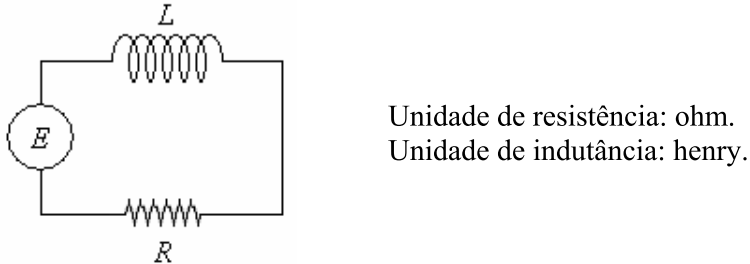
\includegraphics[scale=0.65]{Figs/L1/Resistor.png}\label{fig-resistorL1}
  %   \caption{Representação de um circuito}
  %   \label{Fig:Circ}
  % \end{figure}\\
  % \textbf{Exercício 1:} Se uma bateria de 12 volts é conectada a um circuito em série (como na figura acima) no qual o indutor é de 1/2 henry e o resistor é de 10 ohms, determine o valor da constante $c$ e a corrente $i(t)$. Considere a corrente inicial e o tempo inicial iguais a zero.\\
  % \textbf{Exercício 2:} Determine $\displaystyle\lim_{t\to \infty} i(t)$, sendo $i(t)$ da equação (\ref{eq.resistor})\\
  % \textbf{Exercício 3-Observações:}
  % \begin{enumerate}[a)]
  %   \item O que acontece com o termo $ce^{-\left(\frac{R}{L}\right)t}$ quanto $\displaystyle {t\to \infty}$? \textbf{Explique!} Tal termo é usualmente denominado \textbf{corrente transitória}. \textbf{Explique!}
  %   \item A razão $E/R$ é chamada \textbf{corrente estacionária}. \textbf{Explique!}
  %   \item Após um longo período, a corrente no circuito é governada praticamente pela lei de Ohm $E= Ri $. \textbf{Explique!}
  % \end{enumerate}
  % \begin{resp}
  %   -
  % \end{resp}
\end{questions}

\vspace{1cm}
% \begin{center}
%  \section*{Gabarito}
%\end{center}
\Closesolutionfile{ans}% finaliza a gravação das respostas
\begin{Gabarito}{1}
~
        \begin{multicols}{4}
        \begin{enumerate}[a)]
            \item Finito
            \item Infinito
            \item Finito
            \item Infinito
        \end{enumerate}
    \end{multicols}

    
\end{Gabarito}
\begin{Gabarito}{2}
~
    \begin{multicols}{2}
    \begin{enumerate}[a)]
        \item $A = \{ 4, 5, 6, 7\}$
        \item $B = \{ Abril, Junho, Setembro, Novembro \}$
        \item $C = \{Bras\acute{i}lia\}$
        \item $D = \{ 0, 1, 8\}$
        \item $E = \{0, 1, 2, ...\}$
        \item $F = \{ 0 \}$
        \item $A = \{ 5, 6, 7, ...\}$
        \item $B = \{ 3, 4, 5\}$
    \end{enumerate}
\end{multicols}

\end{Gabarito}
\begin{Gabarito}{3}
~

    \begin{enumerate}[a)]
        \item

        \begin{itemize}
                \item $2 \in A$
                \item Se $n \in A$, então $n^2 \in A$
            \end{itemize}

        \item

            \begin{itemize}
                    \item $a_1 = 1$
                    \item $n \in \mathbb{N+}, a_{n+1} = a_{n} + 2n - 1$
                \end{itemize}

        \item

        \begin{itemize}
                \item $1 \in C$
                \item Se $n \in C$, então $3n \in C$
            \end{itemize}
    \end{enumerate}
\end{Gabarito}
\begin{Gabarito}{4}
~

    \begin{multicols}{4}
        \begin{enumerate}[a)]
            \item V
            \item V
            \item F
            \item V
            \item V
            \item F
            \item F (Operador $\in$ é aplicado a elementos e não a conjuntos)
            \item V
            \item V
            \item F (observar operador)
            \item F
            \item V
        \end{enumerate}
      \end{multicols}
\end{Gabarito}
\begin{Gabarito}{5}
~

    Seja $x \in A$. Então $x \in \mathbb{R}$ e $x^2 - 4x + 3 = 0$ ou $(x - 1)(x - 3) = 0$, o que nos dá $x = 1$ ou $x = 3$. Em qualquer dos casos, $x \in \mathbb{N}$ e $1 \leq x \leq 4$, de modo que $x \in B$. Portanto, $A \subseteq B$. O número 4 pertence a B, mas não pertence a A, logo $A \subset B$.
\end{Gabarito}
\begin{Gabarito}{6}
~

    Sejam $A = \{x | x \in x^2 < 15\}$ e $B = {x | x \in \mathbb{N} e 2x < 7}$.

    Para provar que $A = B$, vamos mostrar que $A \subseteq B$ e $B \subseteq A$. Para $A \subseteq B$, precisamos escolher um elemento arbitrário de A — ou seja, qualquer coisa que satisfaça a propriedade que caracteriza os elementos de A — e mostrar que satisfaz a propriedade que caracteriza os elementos de B. Seja $x \in A$. Então $x$ é um inteiro não negativo que satisfaz a desigualdade $x^2 < 15$. Os inteiros não negativos cujos quadrados são menores do que 15 são 0, 1, 2 e 3, logo esses são os elementos de A. O dobro de cada um desses inteiros não negativos é um número menor do que 7. Portanto, todo elemento de A pertence a B e $A \subseteq B$.

    Vamos mostrar agora que $B \subseteq A$. Todo elemento de B é um inteiro não negativo cujo dobro é menor do que 7. Esses números são 0, 1, 2 e 3, e cada um deles tem o quadrado menor do que 15, logo $B \subseteq A$.
\end{Gabarito}
\begin{Gabarito}{7}
~

    $\wp(A) = \{\emptyset, \{1\}, \{2\}, \{3\}, \{1, 2\}, \{1, 3\}, \{2, 3\}, \{1, 2, 3\}\}$.
\end{Gabarito}
\begin{Gabarito}{8}
~

    $2^n$ elementos.
\end{Gabarito}
\begin{Gabarito}{9}
~

    c
\end{Gabarito}
\begin{Gabarito}{10}
~

    \begin{multicols}{2}
    \begin{enumerate}[a)]
        \item - (anulada) [$A \cup B = \mathbb{N}$]
        \item F
        \item V
        \item - (anulada) [$A \cup C = A$]
        \item V
    \end{enumerate}
\end{multicols}
\end{Gabarito}
\begin{Gabarito}{11}
~

    \begin{multicols}{2}
    \begin{enumerate}[a)]
        \item 10
        \item $\{1,2,3,4,5,7,8,9,10\}$
        \item $\{ 1,2,3 \}$
        \item $\{ 2,8 \}$
        \item $\{ 1,2,3,4,6,7,9 \}$
    \end{enumerate}
\end{multicols}
\end{Gabarito}
\begin{Gabarito}{12}
~

    \begin{multicols}{2}
        \begin{itemize}
            \item $[(A \cup B) \cap C] \cup \left[(A \cup B) \cap \overline{C} \right]$
            \item $(A \cup B) \cap (C \cup \overline{C})$
            \item $(A \cup B) \cap S$
            \item $(A \cup B)$
        \end{itemize}

        \begin{itemize}
            \item (comutatividade)
            \item (distributividade)
            \item (complemento)
            \item (elemento neutro)
        \end{itemize}
    \end{multicols}
\end{Gabarito}
\begin{Gabarito}{13}
~

    $[C \cup (A \cap B)] \cap \left[(A \cap B) \cup \overline{C}\right] = A \cap B$

\end{Gabarito}
\begin{Gabarito}{14}
~

    \begin{multicols}{2}
        \begin{itemize}
            \item $A \cup (B \cap \overline{B})$
            \item $A \cup \emptyset$
            \item $A$
        \end{itemize}

        \begin{itemize}
            \item (distributividade)
            \item (complemento)
            \item (elemento neutro)
        \end{itemize}
    \end{multicols}
\end{Gabarito}
\begin{Gabarito}{15}
~
    \begin{enumerate}[a)]
        \item $\{ -1, 1 \}$
        \item $\{ -3, -2, -1, 0, 1, 2, 3 \}$
        \item $\{{4,8,12,16,20,...} \}$
    \end{enumerate}

\end{Gabarito}
\begin{Gabarito}{16}
~

    \begin{enumerate}[a)]
        \item $\{ x | (\exists y)( y \in \{1,2,3,4\} ~ e ~ x = y^2) \}$
        \item $\{ x | \text{x são os números primos}\}$
        \item $\{{x| \text{x é um inteiro não negativo escrito em forma binária}}\}$
    \end{enumerate}

\end{Gabarito}
\begin{Gabarito}{17}
~

    \begin{center}
        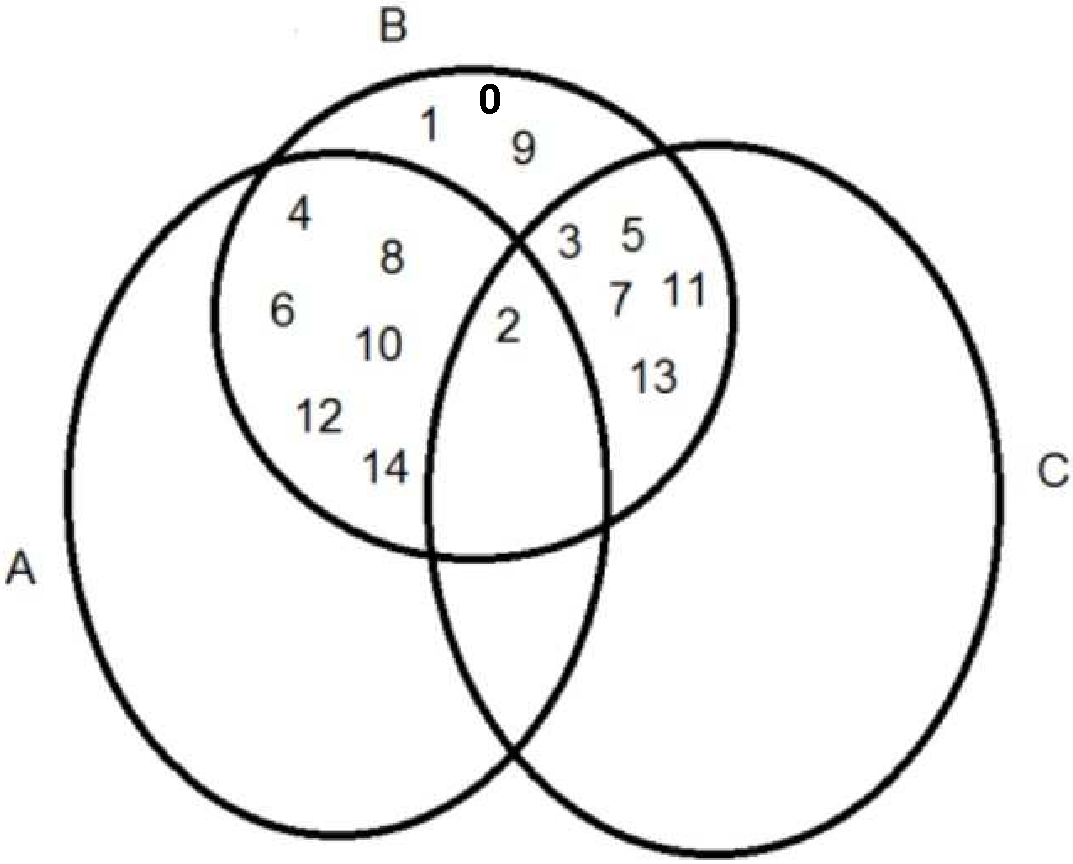
\includegraphics[width=.4\linewidth]{Figs/conjuntos-cropped.pdf}
    \end{center}

\end{Gabarito}
\begin{Gabarito}{18}
~

    \begin{center}
        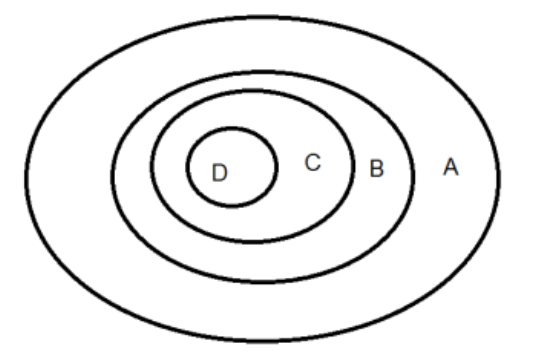
\includegraphics[width=.4\linewidth]{Figs/conjuntos2.png}
    \end{center}
\end{Gabarito}
\begin{Gabarito}{19}
~

    \begin{multicols}{2}
    \begin{enumerate}[a)]
        \item $\{1,2,3,4,5\}$
        \item $\{1,3\}$
        \item $\{5,7,9,11,...\}$
        \item $\{0,5,6,7,8,9,11,13,15,17,...\}$
        \item $\{ 4, 2, \infty\}$
    \end{enumerate}
\end{multicols}

\end{Gabarito}
\begin{Gabarito}{20}
~

    \begin{enumerate}[a)]
        \item $\{(a,x),(a,y),(b,x),(b,y),(c,x),(c,y)\}$
        \item $\{(0,a),(0,b),(0,c),(1,a),(1,b),(1,c)\}$
    \end{enumerate}
\end{Gabarito}
\begin{Gabarito}{21}
~

    \begin{enumerate}[a)]
    \item
    \begin{multicols}{2}
        \begin{itemize}
            \item $A \cup (B \cap \overline{B})$
            \item $A \cup \emptyset$
            \item $A$
        \end{itemize}

        \begin{itemize}
            \item (distributividade)
            \item (complemento)
            \item (elemento neutro)
        \end{itemize}
    \end{multicols}

    \item

    Correção: $A \cap (B \cup \overline{A}) = B \cap A$

    \begin{multicols}{2}
        \begin{itemize}
            \item $(A \cap B) \cup (A \cap \overline{A})$
            \item $(A \cap B) \cup \emptyset$
            \item $(A \cap B)$
            \item $(B \cap A)$
        \end{itemize}

        \begin{itemize}
            \item (distributividade)
            \item (complemento)
            \item (elemento neutro)
            \item (comutatividade)
        \end{itemize}
    \end{multicols}
\end{enumerate}
\end{Gabarito}
\begin{Gabarito}{22}
~

    $A=\{1,3,5,6,7,8,9\}$ e $B=\{2,3,6,9,10\}$
\end{Gabarito}
\begin{Gabarito}{23}
~

    $X=\{1,3,5\}$
\end{Gabarito}
\begin{Gabarito}{24}
~


    a
\end{Gabarito}
 %imprime as soluções
\end{document}
